\subsection{Exemples d'utilisation de Claude}

\begin{bfbox}{La création des \frquote{\textsc{toolbox}}}

    Pour fournir les kits d'outils des exercices de cette formation, j'ai demandé à Claude de me préparer des designs dont je pourrais m'inspirer. 

    J'ai utilisé l'agent scripteur décrit dans cette formation. 

    \begin{tcbenumerate}[2]
        \tcbitem \acc{Le prompt}. \mycomment{On ne s'est pas appliqué. C'est possible grâce à la qualité du pré-prompt.}
        \begin{center}
        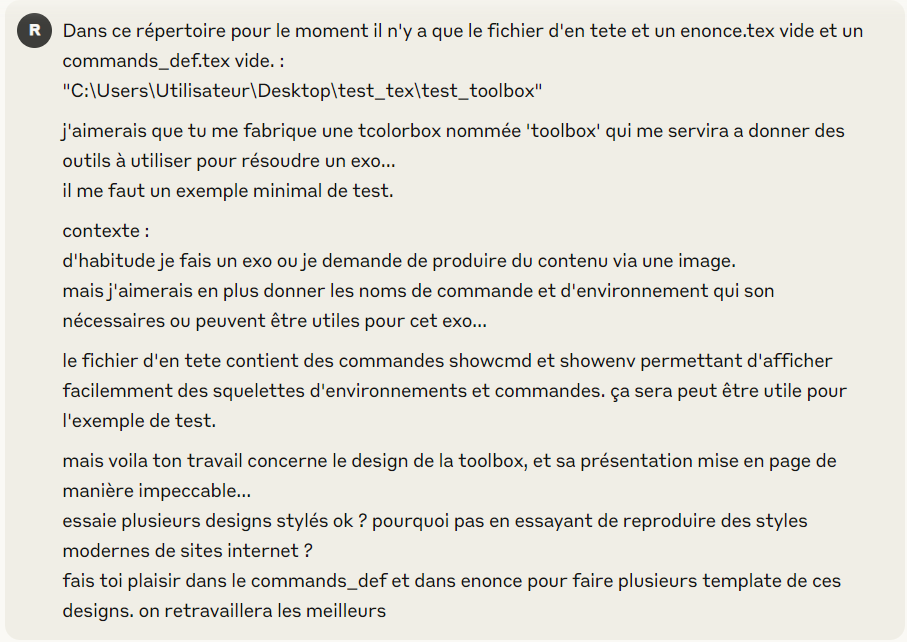
\includegraphics[width=0.75\textwidth]{annexes/Example_craft_toolbox/1.png}
        \end{center}
        
        \tcbitem \acc{L'action}. \mycomment{Le modèle analyse le contenu, puis agis. Il tente même de compiler avec plusieurs compilateurs.}
        \begin{center}
        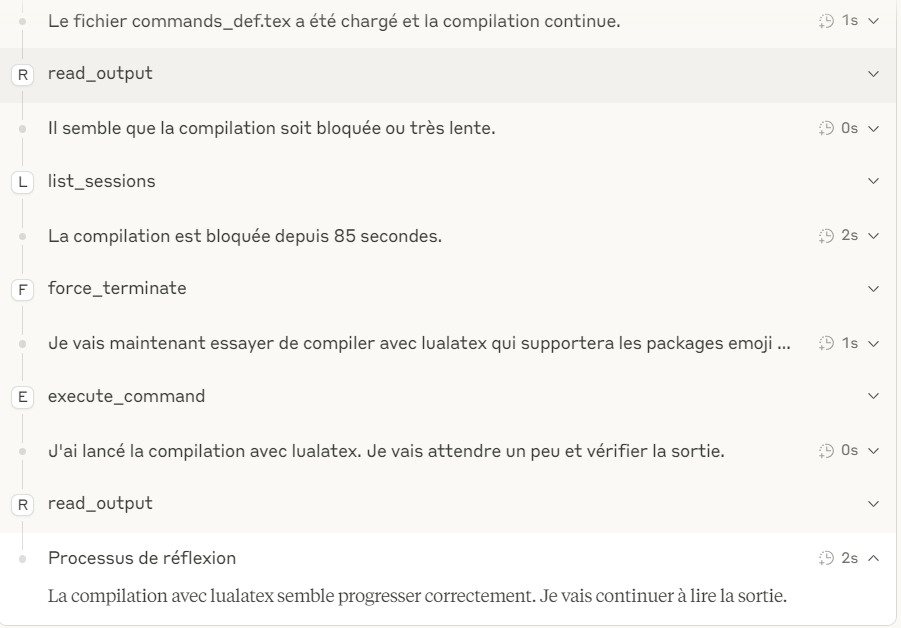
\includegraphics[width=0.75\textwidth]{annexes/Example_craft_toolbox/3.png}
        \end{center}

        \tcbitem \acc{Le rendu}. \mycomment{Claude a été efficace, je n'ai plus qu'à choisir parmi les $8$ exemples fournis.}
        \begin{center}
        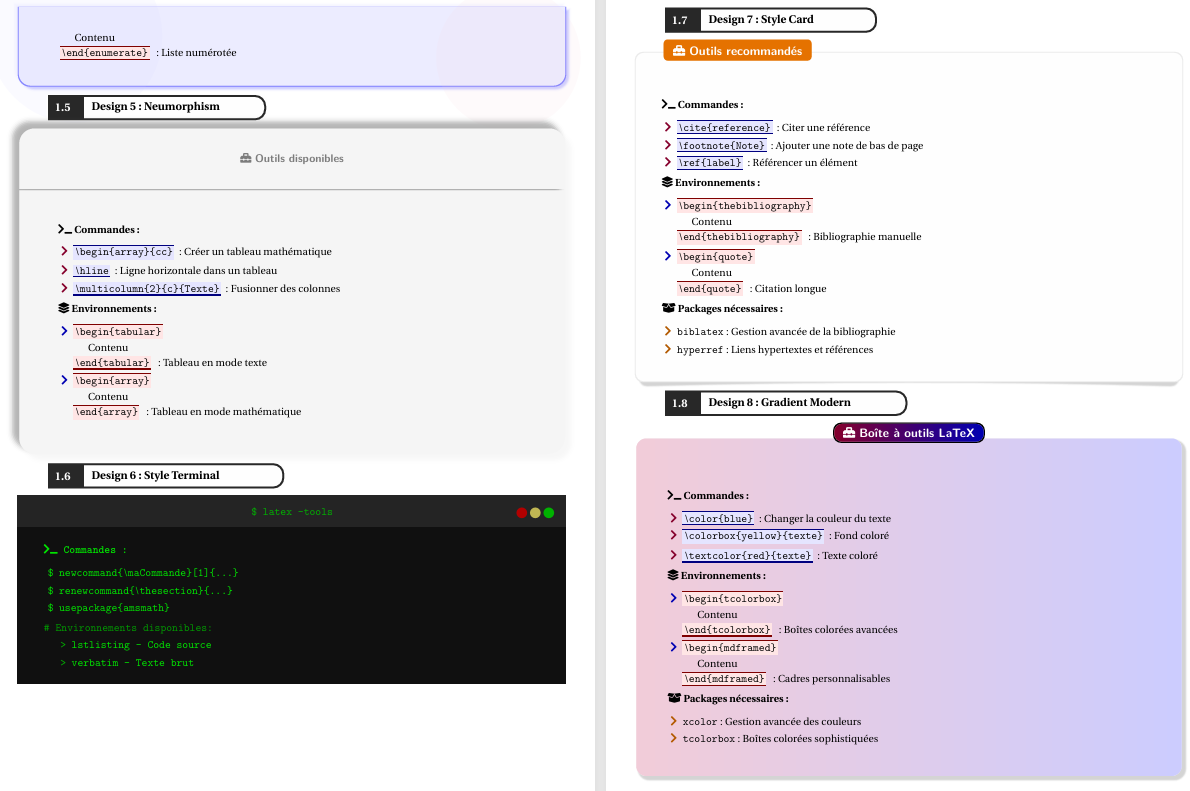
\includegraphics[width=0.75\textwidth]{annexes/Example_craft_toolbox/4.png}
        \end{center}     
        
        \tcbitem \acc{L'investissement en temps} :

        En regardant les propriétés du dossier de test pour ces exemples de design, on a :  
        \begin{itemize}[label=$\bullet$]
            \item \encadrer{Date de création : 8h23}
        
            \item \encadrer[green]{Date de fin d'édition de cet exemple : 9h}
        \end{itemize}

        La création de cet exemple et du design des mes \textsc{toolbox} n'a pris qu'un peu plus d'une demi-heure.
    \end{tcbenumerate}
\end{bfbox}

\begin{bfbox}{Reproduction de contenu}
    Je souhaite adapter un contenu vu sur une ressource à ma façon de procéder. 

    \begin{MultiColonnes}{2}
        \tcbitem Contenu originel :
        
        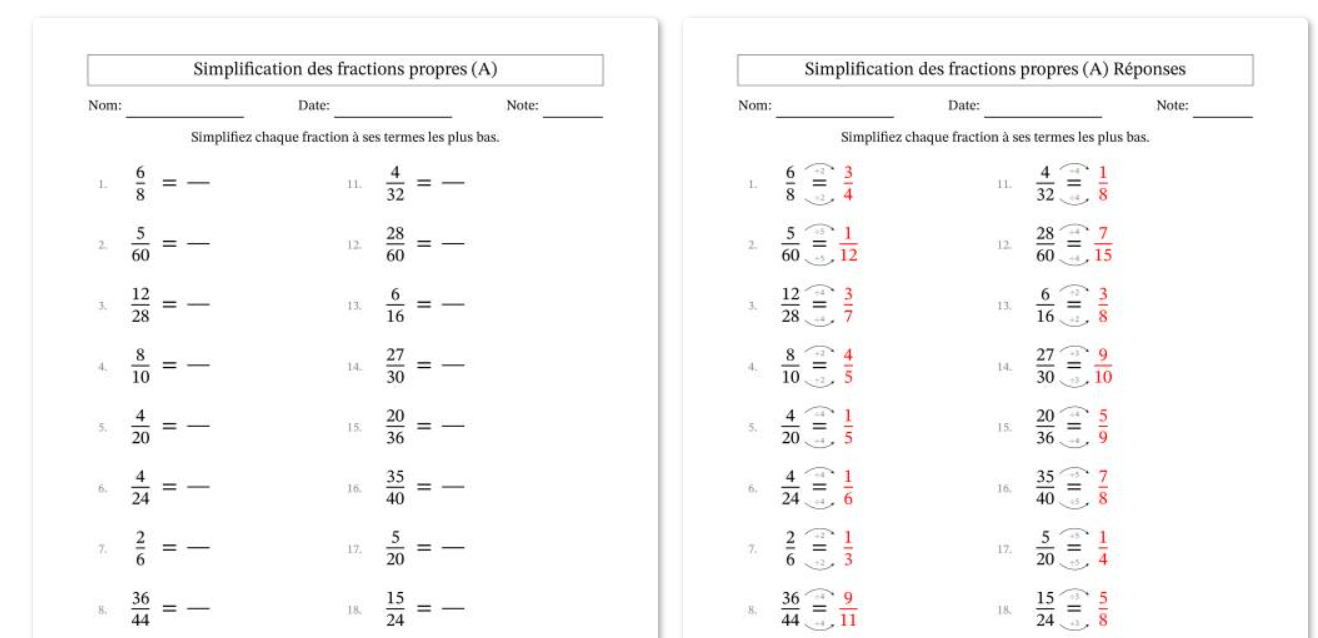
\includegraphics[width=0.75\textwidth]{images/Claude-reproduction/1.png}

        \tcbitem Prompt : 

        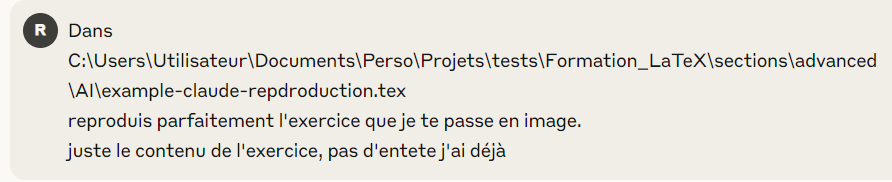
\includegraphics[width=0.75\textwidth]{images/Claude-reproduction/2.png}

        \tcbitem Réaction du modèle : 

        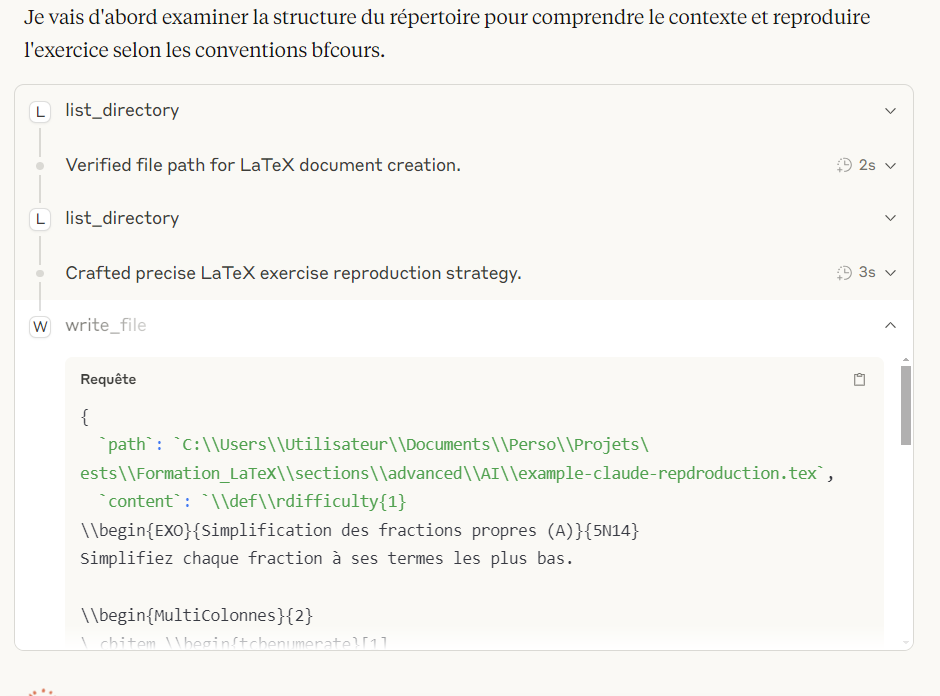
\includegraphics[width=0.55\textwidth]{images/Claude-reproduction/3.png}

        \tcbitem Claude a écrit directement dans un fichier que j'ai inséré ci-dessous.
        
    \end{MultiColonnes}

\end{bfbox}

\def\rdifficulty{1}
\begin{EXO}{Simplification des fractions propres (A)}{5N14}
\acc{Simplifiez} chaque fraction à ses termes les plus bas.

\begin{MultiColonnes}{2}
\tcbitem \begin{tcbenumerate}[1]
    \tcbitem \tcbitempoint{1} $\dfrac{6}{8} = $ \repsim[2cm]{}
    
    \tcbitem \tcbitempoint{1} $\dfrac{5}{60} = $ \repsim[2cm]{}
    
    \tcbitem \tcbitempoint{1} $\dfrac{12}{28} = $ \repsim[2cm]{}
    
    \tcbitem \tcbitempoint{1} $\dfrac{8}{10} = $ \repsim[2cm]{}
    
    \tcbitem \tcbitempoint{1} $\dfrac{4}{20} = $ \repsim[2cm]{}
    
    \tcbitem \tcbitempoint{1} $\dfrac{4}{24} = $ \repsim[2cm]{}
    
    \tcbitem \tcbitempoint{1} $\dfrac{2}{6} = $ \repsim[2cm]{}
    
    \tcbitem \tcbitempoint{1} $\dfrac{36}{44} = $ \repsim[2cm]{}
    
    \tcbitem \tcbitempoint{1} $\dfrac{10}{24} = $ \repsim[2cm]{}
\end{tcbenumerate}

\tcbitem \begin{tcbenumerate}[1][10]
    \tcbitem \tcbitempoint{1} $\dfrac{4}{32} = $ \repsim[2cm]{}
    
    \tcbitem \tcbitempoint{1} $\dfrac{28}{60} = $ \repsim[2cm]{}
    
    \tcbitem \tcbitempoint{1} $\dfrac{6}{16} = $ \repsim[2cm]{}
    
    \tcbitem \tcbitempoint{1} $\dfrac{27}{30} = $ \repsim[2cm]{}
    
    \tcbitem \tcbitempoint{1} $\dfrac{20}{36} = $ \repsim[2cm]{}
    
    \tcbitem \tcbitempoint{1} $\dfrac{35}{40} = $ \repsim[2cm]{}
    
    \tcbitem \tcbitempoint{1} $\dfrac{5}{20} = $ \repsim[2cm]{}
    
    \tcbitem \tcbitempoint{1} $\dfrac{15}{24} = $ \repsim[2cm]{}
\end{tcbenumerate}
\end{MultiColonnes}
\exocorrection

\exocorrection

\begin{MultiColonnes}{2}
\tcbitem \begin{tcbenumerate}[1]
    \tcbitem $\dfrac{6}{8} = \dfrac{3}{4}$
    
    \tcbitem $\dfrac{5}{60} = \dfrac{1}{12}$
    
    \tcbitem $\dfrac{12}{28} = \dfrac{3}{7}$
    
    \tcbitem $\dfrac{8}{10} = \dfrac{4}{5}$
    
    \tcbitem $\dfrac{4}{20} = \dfrac{1}{5}$
    
    \tcbitem $\dfrac{4}{24} = \dfrac{1}{6}$
    
    \tcbitem $\dfrac{2}{6} = \dfrac{1}{3}$
    
    \tcbitem $\dfrac{36}{44} = \dfrac{9}{11}$
    
    \tcbitem $\dfrac{10}{24} = \dfrac{5}{12}$
\end{tcbenumerate}

\tcbitem \begin{tcbenumerate}[1][10]
    \tcbitem $\dfrac{4}{32} = \dfrac{1}{8}$
    
    \tcbitem $\dfrac{28}{60} = \dfrac{7}{15}$
    
    \tcbitem $\dfrac{6}{16} = \dfrac{3}{8}$
    
    \tcbitem $\dfrac{27}{30} = \dfrac{9}{10}$
    
    \tcbitem $\dfrac{20}{36} = \dfrac{5}{9}$
    
    \tcbitem $\dfrac{35}{40} = \dfrac{7}{8}$
    
    \tcbitem $\dfrac{5}{20} = \dfrac{1}{4}$
    
    \tcbitem $\dfrac{15}{24} = \dfrac{5}{8}$
\end{tcbenumerate}
\end{MultiColonnes}

\end{EXO}
